\chapter{Virtualization and Containers}

\section{Introduction}

Virtualization and containers are foundational technologies in modern cloud computing, distributed systems, backend infrastructure, DevOps, and platform engineering.

Almost every large-scale software system today runs inside virtual machines, containers, or both.

Understanding virtualization and containers is essential for Software Development Engineer interviews, Site Reliability Engineering interviews, Cloud Engineering interviews, and Backend Engineering interviews.

\section{Motivation for Virtualization}

Before virtualization became mainstream, applications ran directly on physical servers.

Problems included:

\begin{itemize}
\item Low hardware utilization
\item High infrastructure costs
\item Poor scalability
\item Difficult deployment
\item Resource fragmentation
\end{itemize}

Virtualization addresses these challenges by allowing multiple isolated environments to share the same physical hardware.

Benefits:

\begin{itemize}
\item Better utilization
\item Resource isolation
\item Easier management
\item High availability
\item Scalability
\item Cost reduction
\end{itemize}

\section{Virtual Machines}

A Virtual Machine (VM) is a software emulation of a physical computer.

Each VM includes:

\begin{itemize}
\item Virtual CPU
\item Virtual Memory
\item Virtual Storage
\item Virtual Network Interfaces
\item Guest Operating System
\end{itemize}

\begin{figure}[H]
\centering
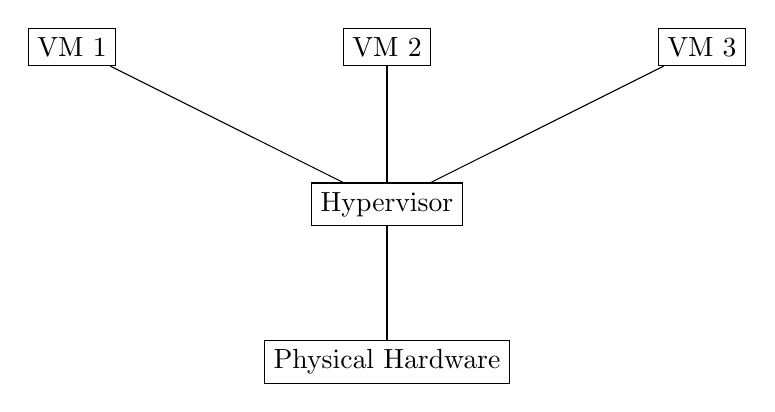
\begin{tikzpicture}
\node[draw] (vm1) at (-4,2) {VM 1};
\node[draw] (vm2) at (0,2) {VM 2};
\node[draw] (vm3) at (4,2) {VM 3};

\node[draw] (hypervisor) at (0,0) {Hypervisor};

\node[draw] (hardware) at (0,-2) {Physical Hardware};

\draw (vm1)--(hypervisor);
\draw (vm2)--(hypervisor);
\draw (vm3)--(hypervisor);
\draw (hypervisor)--(hardware);
\end{tikzpicture}
\caption{Virtual Machine Architecture}
\end{figure}

\section{Hypervisors}

A hypervisor manages virtual machines.

Responsibilities:

\begin{itemize}
\item CPU allocation
\item Memory allocation
\item Device virtualization
\item Scheduling
\item Isolation
\end{itemize}

Examples:

\begin{itemize}
\item VMware ESXi
\item KVM
\item Hyper-V
\item Xen
\item VirtualBox
\end{itemize}

\section{Type 1 Hypervisors}

Type 1 hypervisors run directly on hardware.

\begin{figure}[H]
\centering
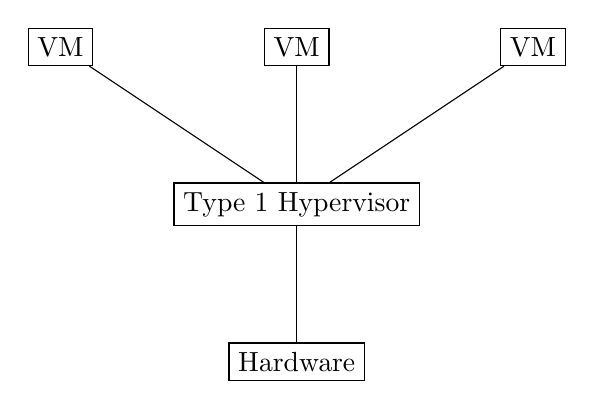
\begin{tikzpicture}
\node[draw] (vm1) at (-3,2) {VM};
\node[draw] (vm2) at (0,2) {VM};
\node[draw] (vm3) at (3,2) {VM};

\node[draw] (hyp) at (0,0) {Type 1 Hypervisor};

\node[draw] (hw) at (0,-2) {Hardware};

\draw (vm1)--(hyp);
\draw (vm2)--(hyp);
\draw (vm3)--(hyp);
\draw (hyp)--(hw);
\end{tikzpicture}
\caption{Type 1 Hypervisor}
\end{figure}

Examples:

\begin{itemize}
\item VMware ESXi
\item Xen
\item Hyper-V
\end{itemize}

Advantages:

\begin{itemize}
\item Better performance
\item Strong isolation
\item Enterprise deployment
\end{itemize}

\section{Type 2 Hypervisors}

Type 2 hypervisors run on a host operating system.

\begin{figure}[H]
\centering
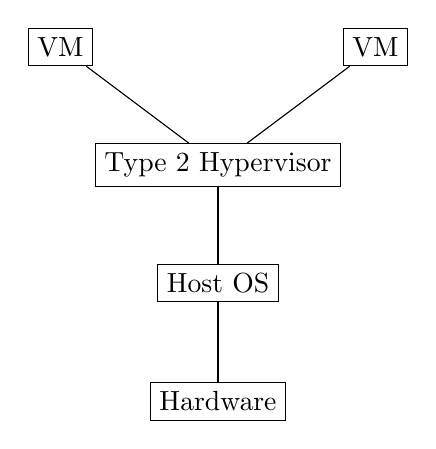
\begin{tikzpicture}
\node[draw] (vm1) at (-2,3) {VM};
\node[draw] (vm2) at (2,3) {VM};

\node[draw] (hyp) at (0,1.5) {Type 2 Hypervisor};

\node[draw] (host) at (0,0) {Host OS};

\node[draw] (hw) at (0,-1.5) {Hardware};

\draw (vm1)--(hyp);
\draw (vm2)--(hyp);
\draw (hyp)--(host);
\draw (host)--(hw);
\end{tikzpicture}
\caption{Type 2 Hypervisor}
\end{figure}

Examples:

\begin{itemize}
\item VirtualBox
\item VMware Workstation
\end{itemize}

\section{Full Virtualization}

Full virtualization completely emulates hardware.

Guest operating systems run unmodified.

Advantages:

\begin{itemize}
\item Compatibility
\item Flexibility
\end{itemize}

Disadvantages:

\begin{itemize}
\item Higher overhead
\end{itemize}

\section{Para-Virtualization}

Guest operating systems are modified to cooperate with the hypervisor.

Advantages:

\begin{itemize}
\item Better performance
\item Lower overhead
\end{itemize}

Disadvantages:

\begin{itemize}
\item Requires guest OS modifications
\end{itemize}

Example:

\begin{itemize}
\item Xen PV
\end{itemize}

\section{Hardware-Assisted Virtualization}

Modern CPUs provide virtualization support.

Examples:

\begin{itemize}
\item Intel VT-x
\item Intel VT-d
\item AMD-V
\item AMD-Vi
\end{itemize}

Benefits:

\begin{itemize}
\item Reduced hypervisor overhead
\item Faster context switching
\item Improved isolation
\end{itemize}

\section{CPU Virtualization}

CPU virtualization allows multiple VMs to share physical processors.

Techniques:

\begin{itemize}
\item Time slicing
\item Virtual CPUs (vCPUs)
\item Hardware support
\end{itemize}

\section{Memory Virtualization}

Memory virtualization provides isolated address spaces.

Techniques:

\begin{itemize}
\item Shadow page tables
\item Nested paging
\item Extended Page Tables (EPT)
\end{itemize}

Benefits:

\begin{itemize}
\item Isolation
\item Security
\item Flexibility
\end{itemize}

\section{Storage Virtualization}

Storage resources are abstracted from physical devices.

Examples:

\begin{itemize}
\item SAN
\item Virtual disks
\item Cloud block storage
\end{itemize}

Advantages:

\begin{itemize}
\item Scalability
\item Simplified management
\end{itemize}

\section{Network Virtualization}

Network virtualization creates logical networks independent of physical topology.

Examples:

\begin{itemize}
\item VLANs
\item SDN
\item Virtual Switches
\item Overlay Networks
\end{itemize}

\section{Containers}

Containers provide lightweight operating-system-level virtualization.

Containers share the host kernel while maintaining isolation.

Advantages:

\begin{itemize}
\item Fast startup
\item Low overhead
\item High density
\item Portability
\end{itemize}

\section{Linux Namespaces}

Namespaces isolate system resources.

Types:

\begin{itemize}
\item PID Namespace
\item Mount Namespace
\item Network Namespace
\item IPC Namespace
\item UTS Namespace
\item User Namespace
\end{itemize}

Example:

A container may see process IDs starting at 1 while the host sees different PIDs.

\section{cgroups}

Control Groups (cgroups) limit and monitor resource usage.

Resources managed:

\begin{itemize}
\item CPU
\item Memory
\item Disk I/O
\item Network bandwidth
\end{itemize}

Example:

\begin{itemize}
\item Limit container memory to 1 GB
\item Restrict CPU usage to two cores
\end{itemize}

\section{Container Isolation}

Container isolation relies on:

\begin{itemize}
\item Namespaces
\item cgroups
\item Capabilities
\item Seccomp
\item AppArmor
\item SELinux
\end{itemize}

\section{Docker Architecture}

Docker is the most popular container platform.

Components:

\begin{itemize}
\item Docker Client
\item Docker Daemon
\item Docker Images
\item Docker Registry
\item Containers
\end{itemize}

\begin{figure}[H]
\centering
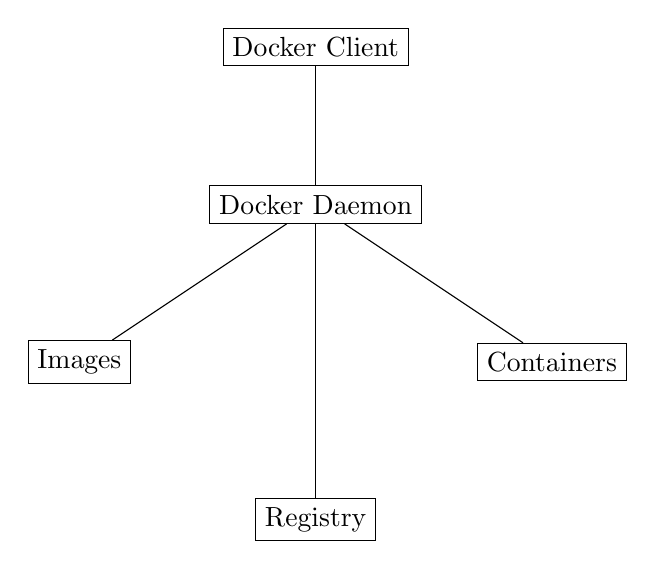
\begin{tikzpicture}
\node[draw] (client) at (0,4) {Docker Client};
\node[draw] (daemon) at (0,2) {Docker Daemon};
\node[draw] (images) at (-3,0) {Images};
\node[draw] (containers) at (3,0) {Containers};
\node[draw] (registry) at (0,-2) {Registry};

\draw (client)--(daemon);
\draw (daemon)--(images);
\draw (daemon)--(containers);
\draw (daemon)--(registry);
\end{tikzpicture}
\caption{Docker Architecture}
\end{figure}

\section{Images}

Images are immutable templates used to create containers.

Characteristics:

\begin{itemize}
\item Layered
\item Read-only
\item Reusable
\end{itemize}

Example:

\begin{lstlisting}[style=interviewcode]
docker pull nginx
\end{lstlisting}

\section{Containers}

Containers are runtime instances of images.

Example:

\begin{lstlisting}[style=interviewcode]
docker run nginx
\end{lstlisting}

Lifecycle:

\begin{itemize}
\item Created
\item Running
\item Paused
\item Stopped
\item Removed
\end{itemize}

\section{Registries}

Container registries store and distribute images.

Examples:

\begin{itemize}
\item Docker Hub
\item Amazon ECR
\item Google Artifact Registry
\item GitHub Container Registry
\end{itemize}

Workflow:

\begin{lstlisting}[style=interviewcode]
docker build
docker push
docker pull
\end{lstlisting}

\section{Kubernetes Overview}

Kubernetes is a container orchestration platform.

Responsibilities:

\begin{itemize}
\item Scheduling
\item Scaling
\item Service discovery
\item Self-healing
\item Rolling updates
\end{itemize}

\section{Pods}

A Pod is the smallest deployable Kubernetes unit.

Characteristics:

\begin{itemize}
\item One or more containers
\item Shared network namespace
\item Shared storage
\end{itemize}

\begin{figure}[H]
\centering
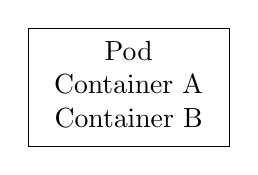
\begin{tikzpicture}
\node[draw] (pod) at (0,0) {
\begin{tabular}{c}
Pod\\
Container A\\
Container B
\end{tabular}
};
\end{tikzpicture}
\caption{Kubernetes Pod}
\end{figure}

\section{Container Scheduling}

Schedulers determine where workloads execute.

Scheduling factors:

\begin{itemize}
\item CPU availability
\item Memory availability
\item Affinity rules
\item Resource requests
\item Taints and tolerations
\end{itemize}

\section{Security Considerations}

Common security concerns:

\begin{itemize}
\item Privileged containers
\item Container escapes
\item Vulnerable images
\item Secret management
\item Supply chain attacks
\end{itemize}

Best practices:

\begin{itemize}
\item Least privilege
\item Image scanning
\item Read-only filesystems
\item Resource limits
\item Network policies
\end{itemize}

\section{Dedicated Interview Section: VM vs Container}

\begin{table}[H]
\centering
\begin{tabular}{lll}
\toprule
Feature & Virtual Machine & Container \\
\midrule
Kernel & Own Kernel & Shared Kernel \\
Startup Time & Seconds/Minutes & Milliseconds \\
Resource Usage & High & Low \\
Isolation & Strong & Moderate \\
Density & Lower & Higher \\
Portability & Good & Excellent \\
\bottomrule
\end{tabular}
\caption{VM vs Container}
\end{table}

\section{Dedicated Interview Section: Docker vs Virtual Machine}

\begin{table}[H]
\centering
\begin{tabular}{lll}
\toprule
Aspect & Docker & VM \\
\midrule
Boot Time & Very Fast & Slower \\
Memory Usage & Low & Higher \\
Kernel Sharing & Yes & No \\
Overhead & Low & High \\
Density & High & Moderate \\
\bottomrule
\end{tabular}
\caption{Docker vs Virtual Machine}
\end{table}

\section{Dedicated Interview Section: How Containers Achieve Isolation}

Containers achieve isolation through:

\begin{enumerate}
\item Namespaces isolate visibility.
\item cgroups isolate resources.
\item Capabilities reduce privileges.
\item Seccomp restricts system calls.
\item AppArmor/SELinux enforce policies.
\end{enumerate}

\begin{figure}[H]
\centering
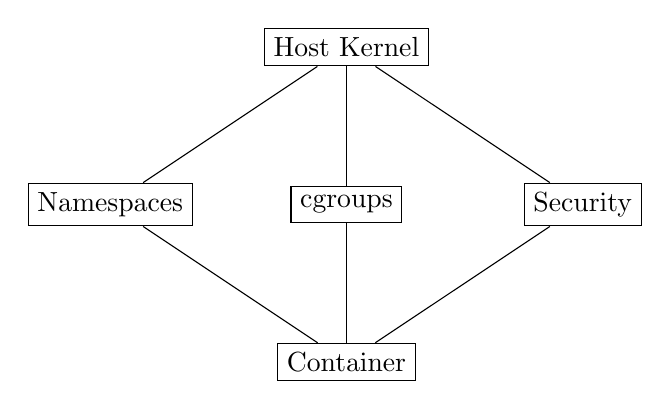
\begin{tikzpicture}
\node[draw] (host) at (0,4) {Host Kernel};

\node[draw] (ns) at (-3,2) {Namespaces};
\node[draw] (cg) at (0,2) {cgroups};
\node[draw] (sec) at (3,2) {Security};

\node[draw] (container) at (0,0) {Container};

\draw (host)--(ns);
\draw (host)--(cg);
\draw (host)--(sec);

\draw (ns)--(container);
\draw (cg)--(container);
\draw (sec)--(container);
\end{tikzpicture}
\caption{Container Isolation Mechanisms}
\end{figure}

\section{Key Takeaways}

\begin{keytakeaways}
Virtualization enables multiple isolated operating systems to share physical hardware through hypervisors. Type 1 hypervisors run directly on hardware while Type 2 hypervisors run on a host operating system. Containers provide lightweight isolation by sharing the host kernel. Linux namespaces provide visibility isolation, while cgroups control resource usage. Docker simplifies container creation and deployment. Kubernetes orchestrates containers at scale. Understanding VM versus container tradeoffs, Docker architecture, Kubernetes concepts, and container isolation mechanisms is essential for modern SDE and backend interviews.
\end{keytakeaways}

\section{Interview Questions with Answers}

\begin{enumerate}
\item What is virtualization?\\
Technology that allows multiple isolated environments to share hardware.

\item What is a virtual machine?\\
A software-emulated computer with its own operating system.

\item What is a hypervisor?\\
Software that manages virtual machines.

\item What is a Type 1 hypervisor?\\
A hypervisor that runs directly on hardware.

\item What is a Type 2 hypervisor?\\
A hypervisor running on top of a host operating system.

\item What is full virtualization?\\
Complete hardware emulation for guest operating systems.

\item What is para-virtualization?\\
Virtualization requiring guest OS awareness.

\item What is hardware-assisted virtualization?\\
CPU-assisted virtualization using features like VT-x and AMD-V.

\item What is CPU virtualization?\\
Sharing physical CPUs among multiple virtual machines.

\item What is memory virtualization?\\
Providing isolated virtual memory spaces.

\item What is storage virtualization?\\
Abstracting physical storage into logical storage resources.

\item What is network virtualization?\\
Creating logical networks independent of hardware.

\item What is a container?\\
A lightweight isolated execution environment sharing the host kernel.

\item What are Linux namespaces?\\
Kernel features providing resource isolation.

\item What are cgroups?\\
Mechanisms for resource accounting and limits.

\item How do containers achieve isolation?\\
Using namespaces, cgroups, and security controls.

\item What is Docker?\\
A containerization platform.

\item What is a Docker image?\\
An immutable template used to create containers.

\item What is a Docker container?\\
A running instance of an image.

\item What is a registry?\\
A repository for container images.

\item What is Kubernetes?\\
A container orchestration system.

\item What is a Pod?\\
The smallest deployable Kubernetes unit.

\item VM or container: which starts faster?\\
Containers.

\item VM or container: which has stronger isolation?\\
Virtual machines.

\item Why are containers popular?\\
Portability, efficiency, and scalability.
\end{enumerate}

\section{MCQs with Answers}

\begin{enumerate}

\item A hypervisor is used to:
\begin{enumerate}[label=(\alph*)]
\item Schedule Threads
\item Manage Virtual Machines
\item Manage Databases
\item Manage Files
\end{enumerate}
Answer: (b)

\item Type 1 hypervisors run:
\begin{enumerate}[label=(\alph*)]
\item On Hardware
\item On Host OS
\item In Containers
\item In BIOS
\end{enumerate}
Answer: (a)

\item VirtualBox is:
\begin{enumerate}[label=(\alph*)]
\item Type 1
\item Type 2
\item Microkernel
\item Container Runtime
\end{enumerate}
Answer: (b)

\item VMware ESXi is:
\begin{enumerate}[label=(\alph*)]
\item Type 1
\item Type 2
\item Docker Runtime
\item Filesystem
\end{enumerate}
Answer: (a)

\item Intel VT-x supports:
\begin{enumerate}[label=(\alph*)]
\item Paging
\item Virtualization
\item Scheduling
\item Journaling
\end{enumerate}
Answer: (b)

\item Containers share:
\begin{enumerate}[label=(\alph*)]
\item Guest Kernel
\item Host Kernel
\item Hypervisor
\item BIOS
\end{enumerate}
Answer: (b)

\item Docker images are:
\begin{enumerate}[label=(\alph*)]
\item Mutable
\item Dynamic
\item Immutable
\item Virtual
\end{enumerate}
Answer: (c)

\item cgroups manage:
\begin{enumerate}[label=(\alph*)]
\item CPU
\item Memory
\item I/O
\item All of the Above
\end{enumerate}
Answer: (d)

\item Namespaces provide:
\begin{enumerate}[label=(\alph*)]
\item Isolation
\item Scheduling
\item Compilation
\item Paging
\end{enumerate}
Answer: (a)

\item Docker containers are created from:
\begin{enumerate}[label=(\alph*)]
\item Registries
\item Images
\item Pods
\item Kernels
\end{enumerate}
Answer: (b)

\item Kubernetes manages:
\begin{enumerate}[label=(\alph*)]
\item Containers
\item Schedulers
\item Nodes
\item All of the Above
\end{enumerate}
Answer: (d)

\item Smallest Kubernetes unit:
\begin{enumerate}[label=(\alph*)]
\item Cluster
\item Node
\item Pod
\item Service
\end{enumerate}
Answer: (c)

\item Full virtualization:
\begin{enumerate}[label=(\alph*)]
\item Requires Modified Guest
\item Emulates Hardware
\item Uses No Hypervisor
\item Uses No CPU
\end{enumerate}
Answer: (b)

\item Para-virtualization:
\begin{enumerate}[label=(\alph*)]
\item Requires Guest Cooperation
\item No Guest Changes
\item No Hypervisor
\item No Memory
\end{enumerate}
Answer: (a)

\item Docker Hub is:
\begin{enumerate}[label=(\alph*)]
\item Hypervisor
\item Registry
\item Scheduler
\item Namespace
\end{enumerate}
Answer: (b)

\item Which provides stronger isolation?
\begin{enumerate}[label=(\alph*)]
\item Container
\item VM
\item Thread
\item Process
\end{enumerate}
Answer: (b)

\item Which starts fastest?
\begin{enumerate}[label=(\alph*)]
\item VM
\item Container
\item BIOS
\item Hypervisor
\end{enumerate}
Answer: (b)

\item Kubernetes scheduling considers:
\begin{enumerate}[label=(\alph*)]
\item CPU
\item Memory
\item Policies
\item All of the Above
\end{enumerate}
Answer: (d)

\item Network namespaces isolate:
\begin{enumerate}[label=(\alph*)]
\item Networks
\item Files
\item Memory
\item Cache
\end{enumerate}
Answer: (a)

\item PID namespaces isolate:
\begin{enumerate}[label=(\alph*)]
\item Process IDs
\item Memory
\item Storage
\item Schedulers
\end{enumerate}
Answer: (a)

\item Storage virtualization abstracts:
\begin{enumerate}[label=(\alph*)]
\item CPUs
\item Physical Storage
\item Schedulers
\item Drivers
\end{enumerate}
Answer: (b)

\item A running image is:
\begin{enumerate}[label=(\alph*)]
\item Registry
\item Pod
\item Container
\item Namespace
\end{enumerate}
Answer: (c)

\item Linux namespaces are:
\begin{enumerate}[label=(\alph*)]
\item Kernel Features
\item Databases
\item Hypervisors
\item Drivers
\end{enumerate}
Answer: (a)

\item cgroups primarily provide:
\begin{enumerate}[label=(\alph*)]
\item Resource Control
\item Networking
\item Compilation
\item Scheduling
\end{enumerate}
Answer: (a)

\item Kubernetes is primarily:
\begin{enumerate}[label=(\alph*)]
\item Hypervisor
\item Orchestrator
\item Database
\item Filesystem
\end{enumerate}
Answer: (b)

\end{enumerate}

\section{Revision Notes}

\begin{revisionnotes}
\item Virtualization enables multiple isolated environments on one machine.
\item Hypervisors manage virtual machines.
\item Type 1 hypervisors run directly on hardware.
\item Type 2 hypervisors run on host operating systems.
\item Full virtualization emulates hardware.
\item Para-virtualization requires guest awareness.
\item Hardware-assisted virtualization uses VT-x and AMD-V.
\item CPU, memory, storage, and network resources can be virtualized.
\item Containers share the host kernel.
\item Namespaces provide isolation.
\item cgroups enforce resource limits.
\item Docker uses images, containers, registries, and a daemon.
\item Images are immutable.
\item Containers are runtime instances of images.
\item Registries distribute images.
\item Kubernetes orchestrates containers.
\item Pods are Kubernetes deployment units.
\item Container scheduling determines workload placement.
\item VM isolation is stronger than container isolation.
\item Containers start significantly faster than virtual machines.
\end{revisionnotes}

\section{Cheat Sheet}

\begin{longtable}{|p{5cm}|p{8cm}|}
\hline
Concept & Summary \\
\hline
Virtualization & Multiple isolated environments on one machine \\
\hline
Virtual Machine & Software-emulated computer \\
\hline
Hypervisor & VM manager \\
\hline
Type 1 Hypervisor & Runs directly on hardware \\
\hline
Type 2 Hypervisor & Runs on host OS \\
\hline
Full Virtualization & Complete hardware emulation \\
\hline
Para-Virtualization & Guest-aware virtualization \\
\hline
VT-x / AMD-V & Hardware-assisted virtualization \\
\hline
CPU Virtualization & Shared CPU resources \\
\hline
Memory Virtualization & Isolated virtual memory \\
\hline
Storage Virtualization & Abstracted storage resources \\
\hline
Network Virtualization & Logical networking \\
\hline
Container & OS-level virtualization \\
\hline
Namespace & Isolation mechanism \\
\hline
cgroup & Resource control mechanism \\
\hline
Docker & Container platform \\
\hline
Image & Immutable template \\
\hline
Container & Running image instance \\
\hline
Registry & Image repository \\
\hline
Docker Hub & Public image registry \\
\hline
Kubernetes & Container orchestrator \\
\hline
Pod & Smallest Kubernetes unit \\
\hline
VM Isolation & Stronger \\
\hline
Container Startup & Faster \\
\hline
Container Security & Namespaces + cgroups + policies \\
\hline
\end{longtable}